%%%%%%%%%%%%%%%%%%%%%%%%%%%%%%%%%%%%%%%%
%Header
%%%%%%%%%%%%%%%%%%%%%%%%%%%%%%%%%%%%%%%%

\documentclass{beamer}
\usepackage{setspace}

\usepackage{amsthm}
\usepackage{latexsym}
\usepackage{natbib}
\usepackage{graphicx} % for figures
\usepackage{epstopdf} % so can use EPS or PDF figures

\setbeamertemplate{footline}{\hfill\insertframenumber/\inserttotalframenumber} 
\setbeamertemplate{footline}[page number]
\usepackage{cmbright}

\usetheme{Frankfurt}


%%%%%%%%%%%%%%%%%%%%%%%%%%%%%%%%%%%%%%%%%%%%%%%%%%%%
%Document starts
%%%%%%%%%%%%%%%%%%%%%%%%%%%%%%%%%%%%%%%%%%%%%%%%%%%%

\begin{document}

\title{Exploratory Data Analysis (EDA) Project}
\subtitle{SPICED Academy}
\author{Pablo Ruiz de Olano}
\date{March 1, 2024}

%%%%%
\begin{frame}
\maketitle
%\titlepage
\end{frame}
%%%%%

%%%%%
\begin{frame}{}

\begin{exampleblock}{Assignment Prompt} 
\emph{``Amy Williams (seller): organized crime type of person, sells several central houses (top 10\%) over time, needs average outskirt houses over time to hide from the FBI.''}
\end{exampleblock} 

\end{frame}
%%%%%

%%%%%
\begin{frame}{Assessing Client's Needs}

Amy would like to: \pause

\begin{itemize}
\item{\textbf{Sell expensive} (top 10\%) houses \textbf{in the city center.}} 
\item{\textbf{Buy cheap} (bottom 90\%) houses \textbf{on the outskirts.}}
\end{itemize} \pause

\

Houses won't be used for living, so \textbf{price} is the \textbf{only relevant factor}. 

\end{frame}
%%%%%

%%%%%
\begin{frame}{Defining Research Questions}

Two different domains: \pause

\begin{itemize}
\item{Expensive houses in the center} 
\item{Cheap houses on the outskirts}
\end{itemize} \pause

\

We want to study the way price evolves:

\begin{itemize}
\item{Geographically} 
\item{Temporally}
\end{itemize}


\end{frame}
%%%%%

%%%%%
\begin{frame}{Geographic Analysis}

Price distribution for all houses in King County: \pause

\begin{center}
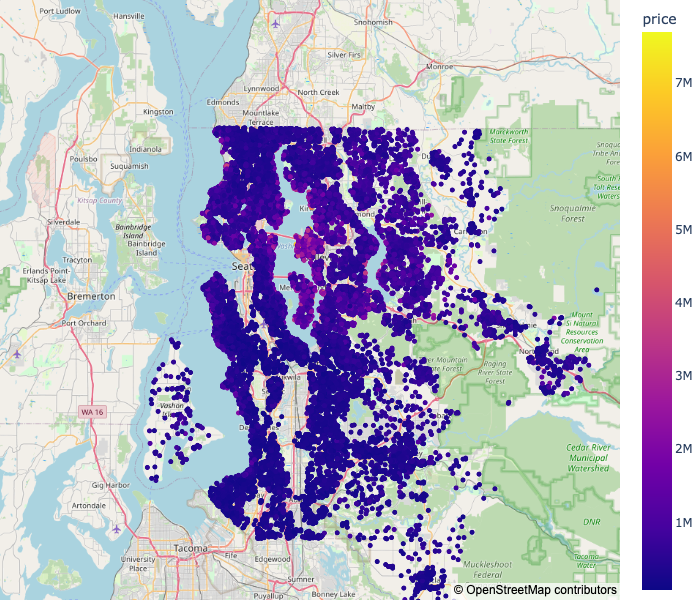
\includegraphics[width=0.6\textwidth]{all_houses_mapbox.png} 
\end{center}

\end{frame}
%%%%%

%%%%%
\begin{frame}{}

But note that there are many more cheap than expensive houses: \pause

\begin{center}
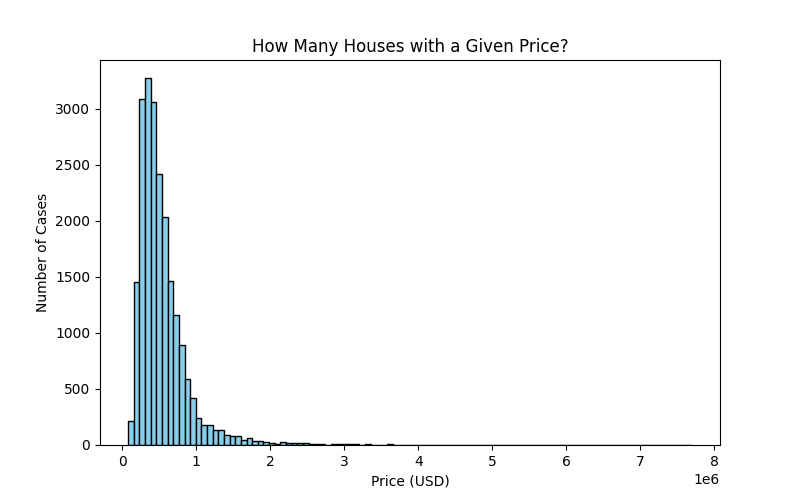
\includegraphics[width=0.9\textwidth]{price_histo.png} 
\end{center}

\end{frame}
%%%%%

%%%%%
\begin{frame}{}

Price distribution for bottom 90\% property: 

\begin{center}
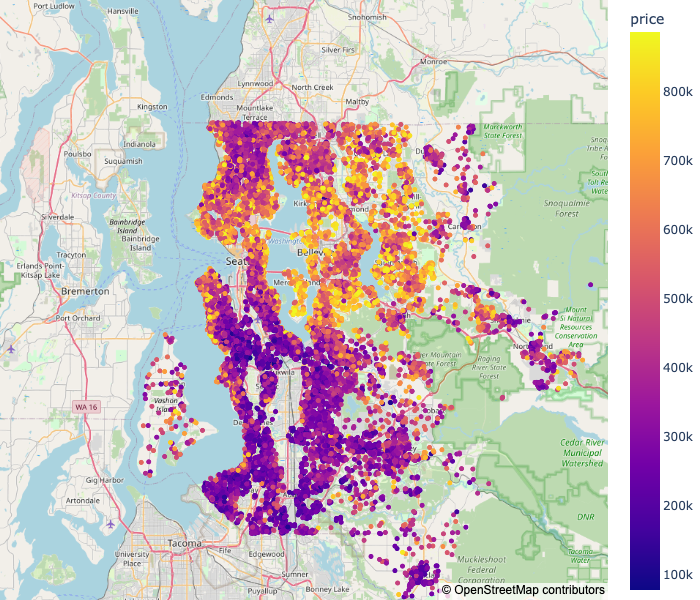
\includegraphics[width=0.7\textwidth]{all_houses_mapbox_clean.png} 
\end{center}

\end{frame}
%%%%%

%%%%%
\begin{frame}{}

Price distribution for top 10\% property in the center: 

\begin{center}
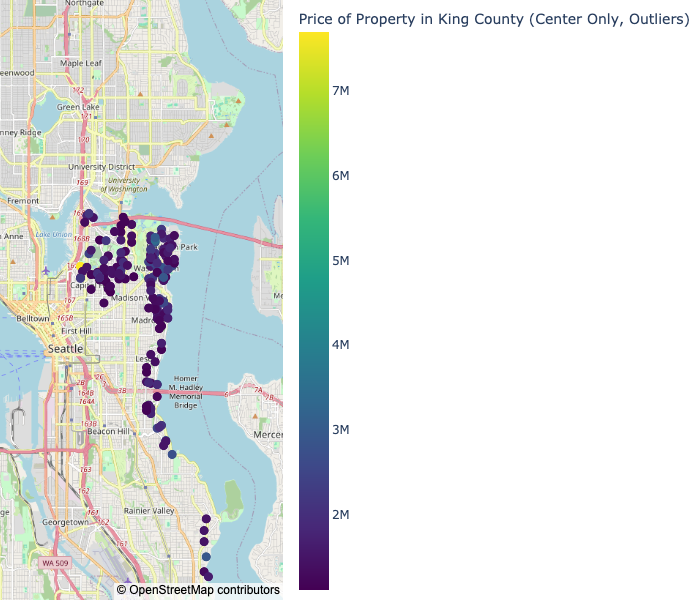
\includegraphics[width=0.7\textwidth]{mapbox_center_outliers.png} 
\end{center}

\end{frame}
%%%%%

%%%%%
\begin{frame}{Temporal Analysis}

Price of housing vs. date of purchase for bottom 90\% property on the outskirts:

\begin{center}
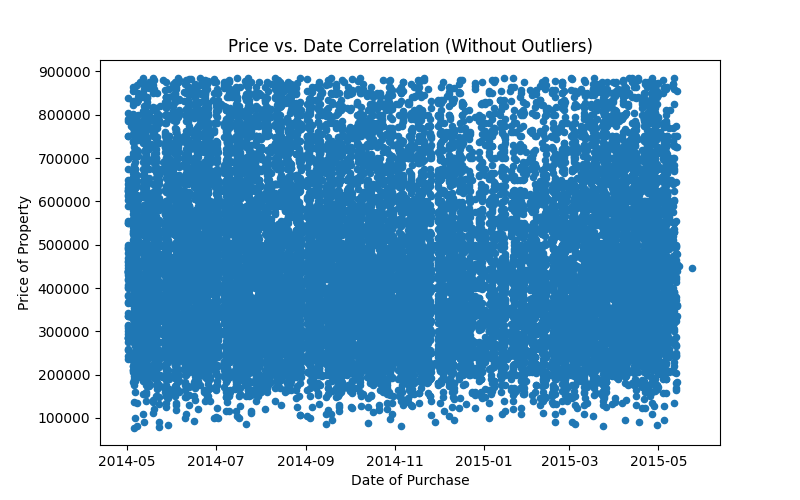
\includegraphics[width=0.85\textwidth]{price_vs_date_cleaned.png} 
\end{center}

\end{frame}
%%%%%

%%%%%
\begin{frame}{}

Price of housing vs. year of construction for top 10\% property in the center:

\begin{center}
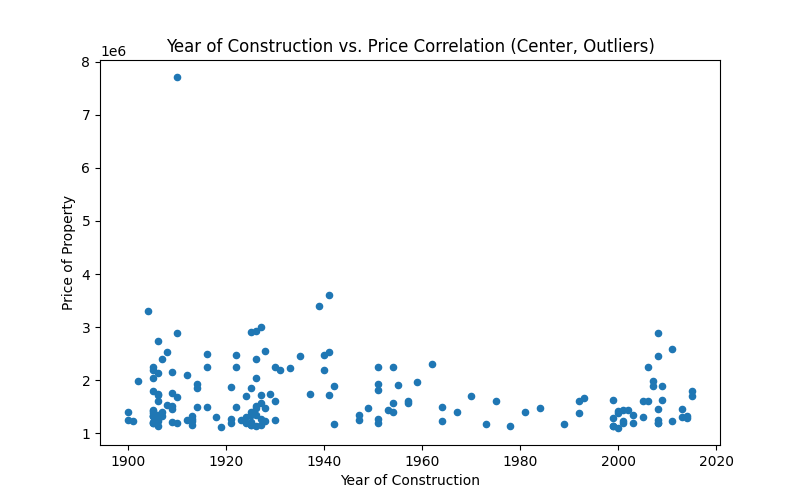
\includegraphics[width=0.85\textwidth]{construction_vs_price_center_outliers.png} 
\end{center}

\end{frame}
%%%%%

%%%%%
\begin{frame}{Insights}
\pause
Geographic insights:

\begin{itemize}
\item{\textbf{Most expensive} property in central Seattle is located on the \textbf{west shore} of Lake Washington and in northern downtown.}
\item{\textbf{Cheapest} property on the outskirts is located in the \textbf{southern part} of the King County.} \pause
\end{itemize}

Temporal insights (tentative): patterns are \textbf{independent of}:
\begin{itemize}
\item{The \textbf{date of purchase} of the property.}
\item{The \textbf{year of construction} of the property.}
\end{itemize} 


\end{frame}
%%%%%

%%%%%
\begin{frame}{Recommendations}

Selling and buying tips for Amy:

\begin{itemize}
\item{Central property on the West Shore of Lake Washington should only be sold at a very high price (minimum $\$$2M).}
\item{Purchase strategy should focus on south of the county.}
\item{Property in the southern part of King County should be bought at a very low price only (maximum $\$$400k).}
\item{No rush to sell or buy, at least within the next year, since price is likely to remain constant (tentative).}
\item{Further research recommended to clarify time dependence.}
\end{itemize}

\end{frame}
%%%%%


\end{document}

